%!TEX root = main.tex
\newpage
\thispagestyle{plain}

\chapter{Plán práce na diplomovom projekte}

\section{Plán práce na diplomovom projekte I}

Prácu na diplomovom projekte I sme navrhli a naplánovali nasledovne:

\begin{table}[h]
\centering
\caption{Plán práce na diplomovom projekte I}
\begin{tabular}{|m{2.3cm}|m{12cm}|}
\hline
1-5.~týždeň semestra   & Analýza problematiky odporúčania v kontexte CQA systémov a súčasného výskumu v tejto oblasti. \\ \hline
6-7.~týždeň semestra   & Analýza dostupných dát na platforme Stack Exchange a možností verejného API platformy. \\ \hline
8-9.~týždeň semestra   & Vytvorenie predbežného návrh metódy riešenia problému a návrh metód overenia výsledkov. \\ \hline
10-12.~týždeň semestra & Spísanie správy diplomového projektu I v rátane analýzy a predbežného návrhu riešenia a overenia. \\ \hline
\end{tabular}
\end{table}

\textbf{Zhodnotenie}\\
Navrhnutý plán práce v rámci diplomového projektu I sa nám do veľkej miery podarilo dodržať. Časový sklz sa prejavil až
vo fáze návrhu metódy riešenia problému, čím sa posunulo spísanie správy až do 11. týždňa semestra.

\newpage
\section{Plán práce na diplomovom projekte II}

\begin{table}[h]
\centering
\caption{Plán práce na diplomovom projekte II}
\begin{tabular}{|m{2.3cm}|m{12cm}|}
\hline
1-2.~týždeň semestra   & -- Príprava databázy a aktualizačného modulu.
				\newline -- Vytvorenie modelov pre získavanie spätnej väzby od používateľov.
				\newline -- Prvotná dátová analýza.
				\\ \hline
3-4.~týždeň semestra   & -- Príprava rozhrania pre odoberanie informačných bulletinov.
				\newline -- Generovanie informačných bulletinov na základe prvotného modelu.
				\newline -- Nasadenie systému a otestovanie v reálnych podmienkach.
				\\ \hline
5-8.~týždeň semestra   & -- Získavanie používateľov informačného bulletinu.
				\newline -- Spracovanie dát, vytvorenie reálnych modelov používateľov a otázok, generovanie odporúčaní.
				\newline -- Príprava metód diverzifikácie odporúčaní.
				\newline -- Písanie diplomovej práce.
				\\ \hline
9-12.~týždeň semestra  & -- Overenie a vyhodnocovanie informačných bulletinov.
				\newline -- Nasadenie a porovnanie metód diverzifikácie.
				\newline -- Počiatočné overenie výsledkov.
				\newline -- V prípade neúspechu online experimentu, plánovanie offline expermientov.
				\\ \hline
\end{tabular}
\end{table}

\textbf{Zhodnotenie}\\
Navrhnutý plán práce v rámci diplomového projektu I sa nám do značnej miery podarilo dodržať. Príprava a implementácia
infraštruktúry systému StackLetter však zabrala viac času, ako sme predpokladali, takže došlo k určitému časovému sklzu.
Voči verzii z DP1 sme tiež prepracovali návrh metódy diverzifikovaného odporúčania. Samotnú implementáciu
odporúčania a~diverzifikácie sme posunuli do nasledujúceho letného semestra. Celkovo sme s aktuálnym stavom spokojní,
napriek tomu, že sme nedodržali predpokladaný plán, keďže sa implementácia infraštruktúry a kooperácia s externými
systémami Stack Exchange ukázala náročnejšia, ako boli naše predpoklady.

\newpage
\section{Plán práce na diplomovom projekte III}\label{apx:dp3plan}

\begin{table}[h]
\centering
\caption{Plán práce na diplomovom projekte III}
\begin{tabular}{|m{2.3cm}|m{12cm}|}
\hline
1-2.~týždeň semestra & -- Pokračovanie online nekontrolovaného experimentu.
			  \newline -- Spracovanie dát, vytvorenie modelov používateľov a otázok. \\ \hline
3-4.~týždeň semestra & -- Príprava metódy proporčnej diverzifikácie odporúčaní
			  \newline -- Vyhodnotenie úspechu/neúspechu online experimentu \\ \hline
5-6.~týždeň semestra & -- Príprava metódy diverzifikácie prostedníctvom tématického vzorkovania
              \newline -- V prípade neúspechu online experimentu, príprava kontrolovaného experimentu \\ \hline
7-8.~týždeň semestra & -- Vyhodnocovanie výsledkov experimentov
			  \newline -- Písanie diplomovej práce \\ \hline
9-10.~týždeň semestra & -- Písanie diplomovej práce \\ \hline
\end{tabular}
\end{table}

\textbf{Zhodnotenie}\\
Navrhnutý plán práce v rámci diplomového projektu III sa nám podarilo dodržať. Online experiment bol úspešný, preto nebolo
potrebné pripravovať kontrolovaný experiment.

\afterpage{\blankpage}
\newpage
\chapter{Technická dokumentácia systému}\label{tech-doc}

\section{Modul pre registráciu nových používateľov}

Tento modul predstavuje webovú aplikáciu určenú na registráciu nových používateľov systému StackLetter. Implementovaná je
v jazyku PHP 7.1 s použitím MVC/MVP webového frameworku Nette 2.4. Ďalej popisujeme niektoré dôležité komponenty tohto modulu.

\textbf{HomepagePresenter}\\
Táto trieda zabezpečuje hlavnú funkcionalitu stránky -- autentifikáciu a registráciu používateľov, ako aj manažment
používateľského konta. Autentifikácia používateľa sa vykonáva prostredníctvom Stack Exchange API s využitím protokolu OAuth 2.0.
Zabezpečuje tiež funkcionalitu kontaktného formuláru.

\textbf{SubscriptionPresenter}\\
Spolu s príslušnou modelovou triedou \textit{SubscriptionModel} implementuje možnosť odhlásenia sa z odoberania
informačného bulletinu, generovanie \textit{unsubscribe} odkazov pre jednotlivé informačné bulletiny, zbieranie spätnej
väzby po odhlásení sa z odoberania a možnosť opätovného prihlásenia sa.

\textbf{AsyncJobProcessor}\\
Táto trieda zabezpečuje asynchrónne spracovanie dlhotrvajúcich úloh. Vďaka asynchrónnemu spracovaniu týchto úloh ostáva
odozva používateľského rozhrania rýchla. Konkrétne vykonáva odoslanie uvítacieho e-mailu používateľovi po úspešnej
registrácii prostredníctvom služby SendGrid s využitím protokolu SMTP, a následné stiahnutie používateľského profilu
prostredníctvom Stack Exchange API.
Samotná webová aplikácia zadáva tomuto komponentu úlohy na asynchrónne spracovanie prostredníctvom Redis fronty.


\section{Modul pre generovanie a odosielanie informačných bulletinov}

Tento modul je zodpovedný za samotné zostavovanie a odosielanie informačných bulletinov jednotlivým zaregistrovaným
používateľom. Skladá sa z dvoch samostatných častí -- komponentu na zostavovanie informačných bulletinov a komponentu
na odosielanie informačného bulletinu. Oba komponenty medzi sebou asynchrónne komunikujú prostredníctvom Redis fronty.

Modul je navrhnutý genericky, aby nebolo potrebné do neho zasahovať v prípade pridania nových sekcií informačných bulletinov,
prípadne nových typov obsahu. Pre každý typ obsahu je potrebné iba definovať HTML šablónu.

Všetky hypertextové odkazy, ktoré sa nachádzajú v informačnom bulletine, smerujú na evaluačný modul, ktorý prostredníctvom
kliknutí na odkazy zaznamenáva používateľovu implicitnú a explicitnú spätnú väzbu a následne je používateľ presmerovaný
na reálny cieľ odkazu. Každý informačný bulleitn tiež obsahuje tzv. sledovací pixel (angl.~\textit{tracking pixel}), čo je
transparentný obrázok veľkosti 1x1 pixelov, načítavaný externe z evaluačného modulu, ktorý nám umožňuje detekovať otvorenie informačného
bulletinu používateľom.

\textbf{Builder -- komponent pre zostavovanie informačného bulletinu}
\begin{my_enumerate}
\item{Prostredníctvom \textit{cronu} sa tento komponent spúšťa každý deň pre vygenerovanie denných informačných bulletinov,
ako aj raz za týždeň pre generovanie týždenných bulletinov.}
\item{Na základe zvolenej frekvencie sa vyberie zoznam používateľov, pre ktorých sa budú generovať bulletiny.}
\item{Prostredníctvom REST API si komponent vyžiada štruktúru bulletinu pre daného používateľa. Odpoveď obsahuje zoznam
sekcií, ich nadpis a popis, ako aj URL adresu REST API koncového bodu, ktorý má pre danú sekciu vrátiť obsah.}
\item{Prostredníctvom REST API si komponent vyžiada zoznam otázok (alebo iného obsahu) pre jednotlivé sekcie
informačného bulletinu.}
\item{Následne komponent zostaví kompletnú štruktúru celého informačného bulletinu so všetkými sekciami a ich obsahom,
a túto štruktúru odovzdá šablónovaciemu komponentu, ktorý zostaví výsledný HTML kód informačného bulletinu.}
\item{Informácia o vygenerovaní nového informačného bulletinu sa vloží do Redis fronty, kde čaká na odoslanie.}
\end{my_enumerate}

\textbf{Mailer -- komponent pre odosielanie informačného bulletinu}\\
Tento komponent postupne vyberá z Redis fronty zoznam vygenerovaných informačných bulletinov, a využívajúc SMTP API služby
SendGrid odosiela používateľom jednotlivé informačné bulletiny, na ktorých odoberanie sa prihlásili.
Tento komponent je spustený na serveri ako služba, a je k dispozícii neustále.

\begin{figure}[H]\begin{center}
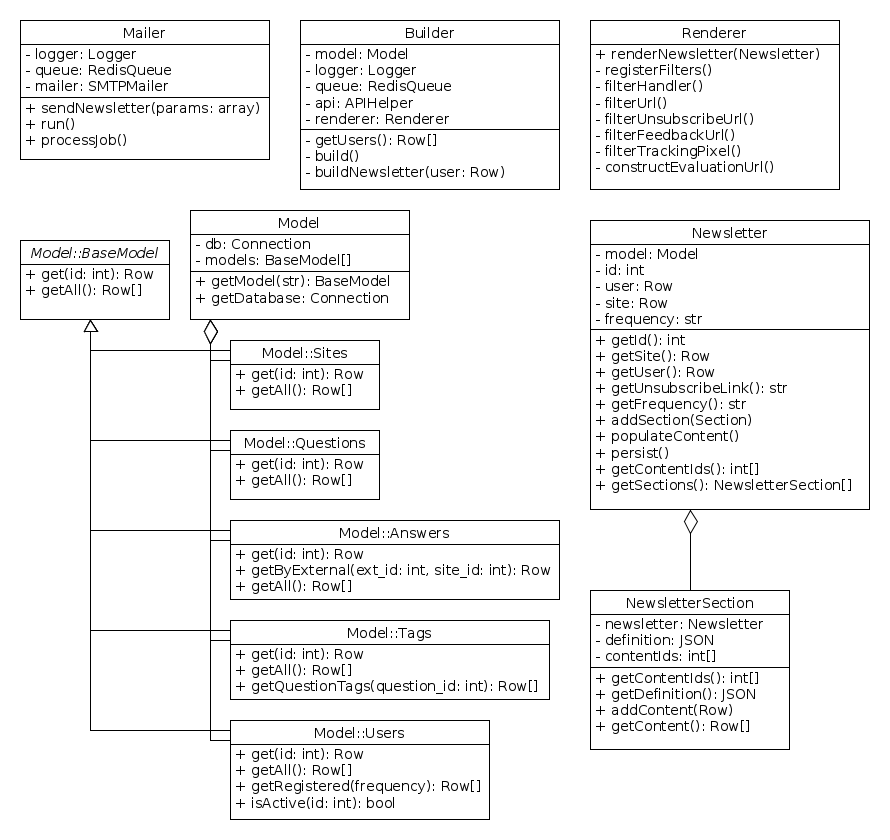
\includegraphics[scale=0.355]{mailer-schema}
\caption{Schéma modulu pre generovanie a odosielanie informačných bulletinov \label{fig:mailer-schema}}\end{center}
\end{figure}

\section{Modul pre spracovanie statickej zálohy databázy}

Tento modul číta \textit{XML dump} Stack Exchange databázy a generuje príkazy SQL dialektu PostgreSQL pre uloženie dát
do databázového modelu systému StackLetter (príloha~\ref{apx:dbmodel}). Zároveň tiež vykonáva konverziu mapovania jednotlivých
entít zo Stack Exchange reprezentácie.

Import dát je vykonávaný dávkovo a v poradí podľa závislostí jednotlivých entít -- najprv sa importujú používatelia,
následne otázky, odpovede, komentáre, značky a nakoniec odznaky.


\section{Modul pre personalizované odporúčanie}
Tento modul je zodpovedný za vytváranie zoznamov odporúčaní pre jednotlivé sekcie personalizovaného informačného bulletinu.
Je implementovaný v jazyku Python 3, a poskytuje REST API pre modul pre generovanie a odosielanie informačných bulletinov.
Modul sa skladá z troch základných komponentov -- \textit{recommender, profiles, train} -- a viacerých pomocných komponentov
-- \textit{db, queries, utils}.

\textbf{Komponent Profiles}\\
Tento komponent obsahuje implementácie profilu otázok a používateľského profilu, ako aj odvodený komunitný profil.
Jednotlivé profily sú implementované v samostatných triedach.

\textbf{Komponent Recommender}\\
Komponent obsahuje implementáciu oboch odporúčacích metód v samostatných triedach -- personalizované odporúčanie,
aj odporúčanie s diverzifikačnou metódou tématického vzorkovania.

\textbf{Kompontent Train}\\
Obsahuje implementáciu funkcionality pre aktualizáciu používateľských modelov, ktorá sa vykonáva pravidelne prostredníctom
nástroja \textit{cron}.

Ostatné komponenty obsahujú podporné funkcie a funkcie pre prácu s databázou, ako aj konfiguráciu REST API, ktoré tento
modul poskytuje.

\section{Databázový model}\label{apx:dbmodel}
\begin{figure}[H]\begin{center}
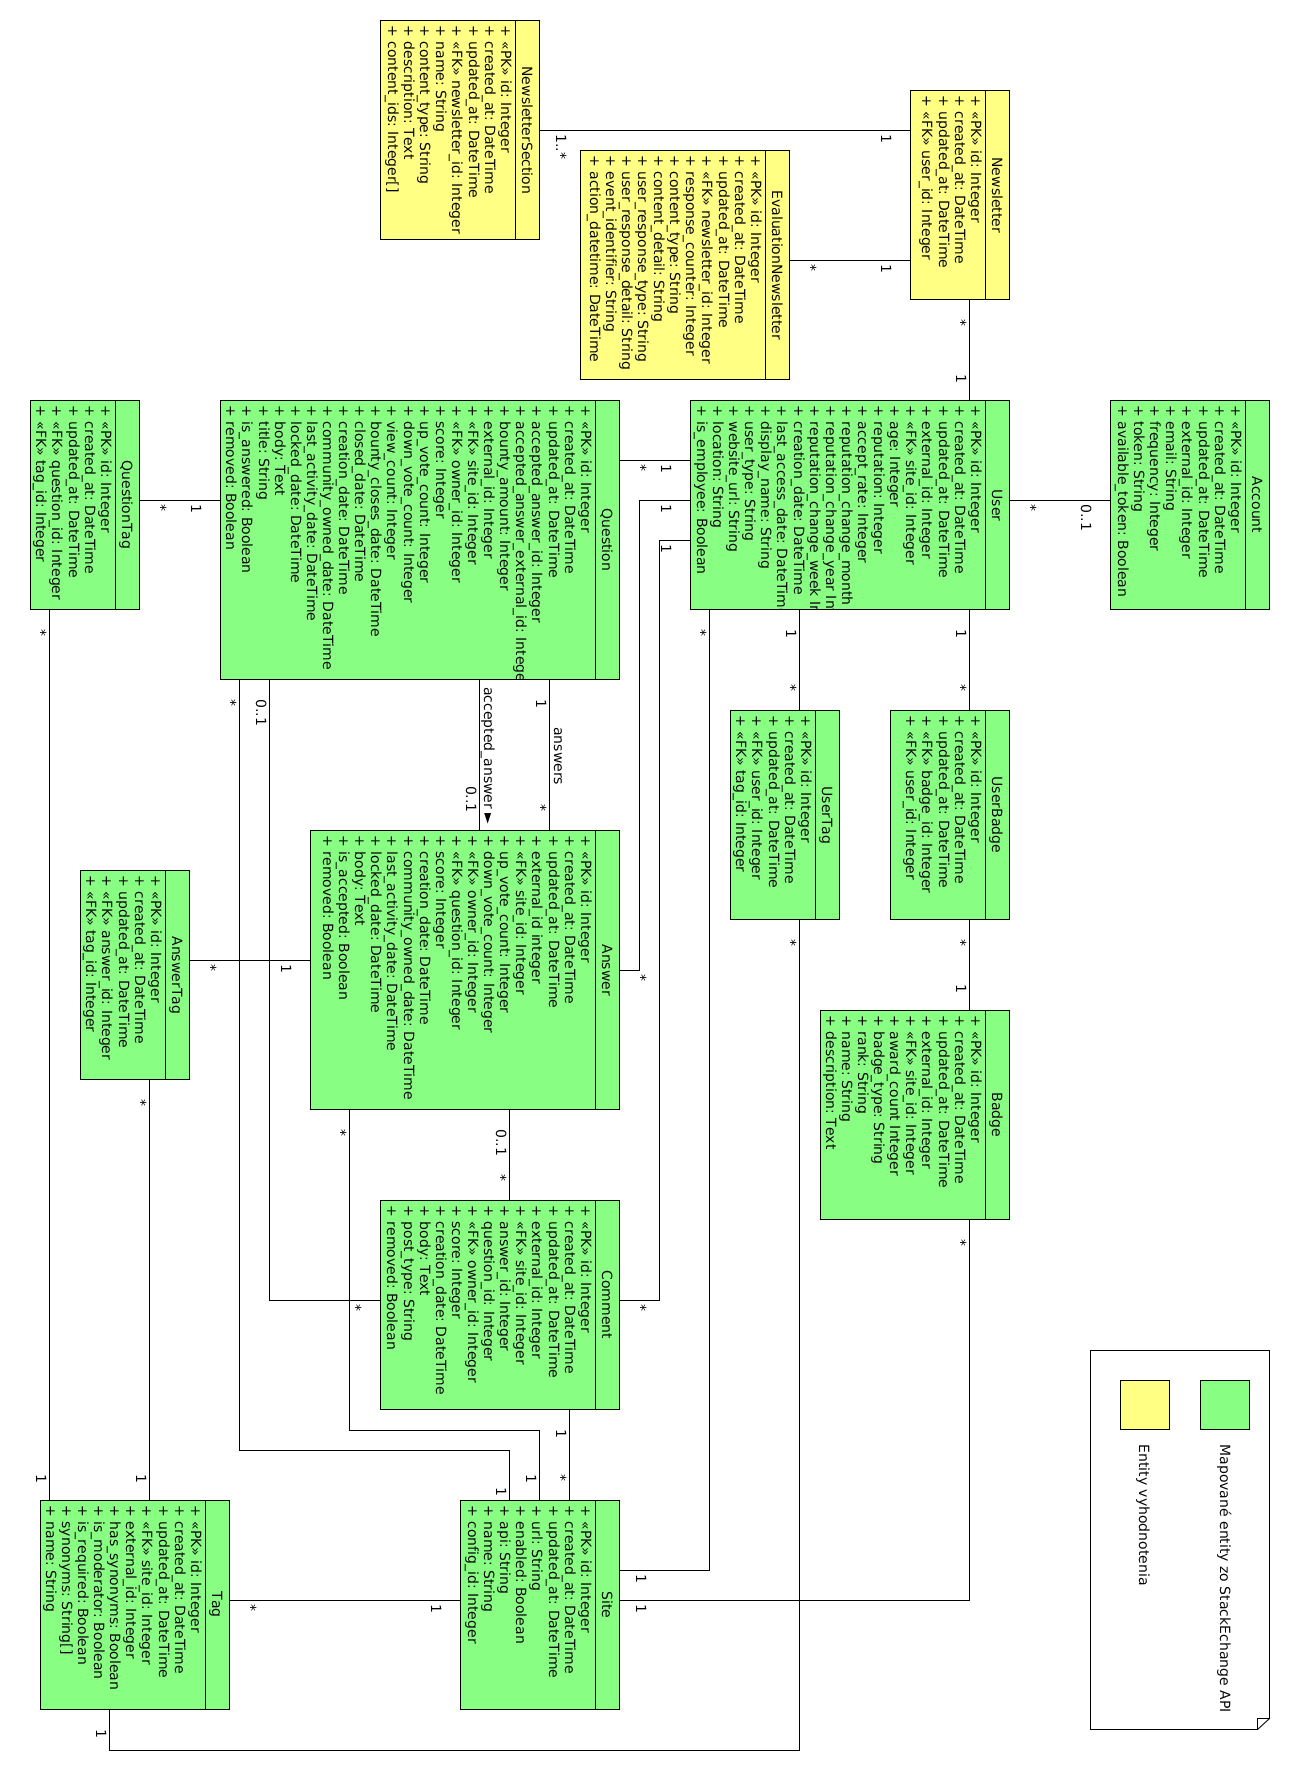
\includegraphics[scale=0.355]{db-model}
\caption{Databázový model systému StackLetter.\label{fig:db-model}}\end{center}
\end{figure}

\afterpage{\blankpage}
\newpage
\chapter{Inštalačná príručka}

\textbf{Závislosti systému}\\
1. Python 3.6+, PIP, VirtualEnv\\
2. PHP 7.1+, Composer\\
3. PostgreSQL server 9.6+\\
4. Redis server 2.8+\\
5. Nginx server 1.6+\\
6. Git 2.1+

\textbf{Inštalácia modulu pre registráciu nových používateľov}\\
Inštalácia prebieha prostredníctvom nástroja Composer -- správcu balíčkov pre jazyk PHP. Po inštalácii je potrebné nastaviť
parametre v konfiguračnom súbore \textit{app/config/config.local.neon}.

\lstset{language=nil}
\begin{lstlisting}
$ git clone https://github.com/StackLetter/LandingPage.git .
$ composer install
\end{lstlisting}

\textbf{Inštalácia modulu pre generovanie a odosielanie informačných bulletinov}\\
Inštalácia prebieha prostredníctvom nástroja Composer -- správcu balíčkov pre jazyk PHP. Po inštalácii je potrebné nastaviť
parametre v konfiguračnom súbore \textit{config/local.neon}.

\begin{lstlisting}
$ git clone https://github.com/StackLetter/Mailer.git .
$ composer install
\end{lstlisting}

\textbf{Inštalácia modulu pre spracovanie statickej zálohy databázy}\\
Inštalácia prebieha prostredníctvom nástroja Composer -- správcu balíčkov pre jazyk PHP. Po inštalácii je potrebné nastaviť
parametre v konfiguračných súboroch \textit{config.json, config.db.json}.

\begin{lstlisting}
$ git clone https://github.com/StackLetter/DumpImport.git .
$ composer install
\end{lstlisting}

\textbf{Inštalácia modulu pre personalizované odporúčanie}\\
Inštalácia prebieha prostredníctvom nástroja PIP -- správcu balíčkov pre jazyk Python. Po inštalácii je potrebné nastaviť
parametre v konfiguračnom súbore \textit{recommender/config.py}.

\begin{lstlisting}
$ git clone https://github.com/StackLetter/Recommender.git .
$ virtualenv env
$ env/bin/pip install -r requirements.txt
\end{lstlisting}


\afterpage{\blankpage}
\newpage
\chapter{Výsledky dotazníku odoberateľov}
\label{appendix:survey}
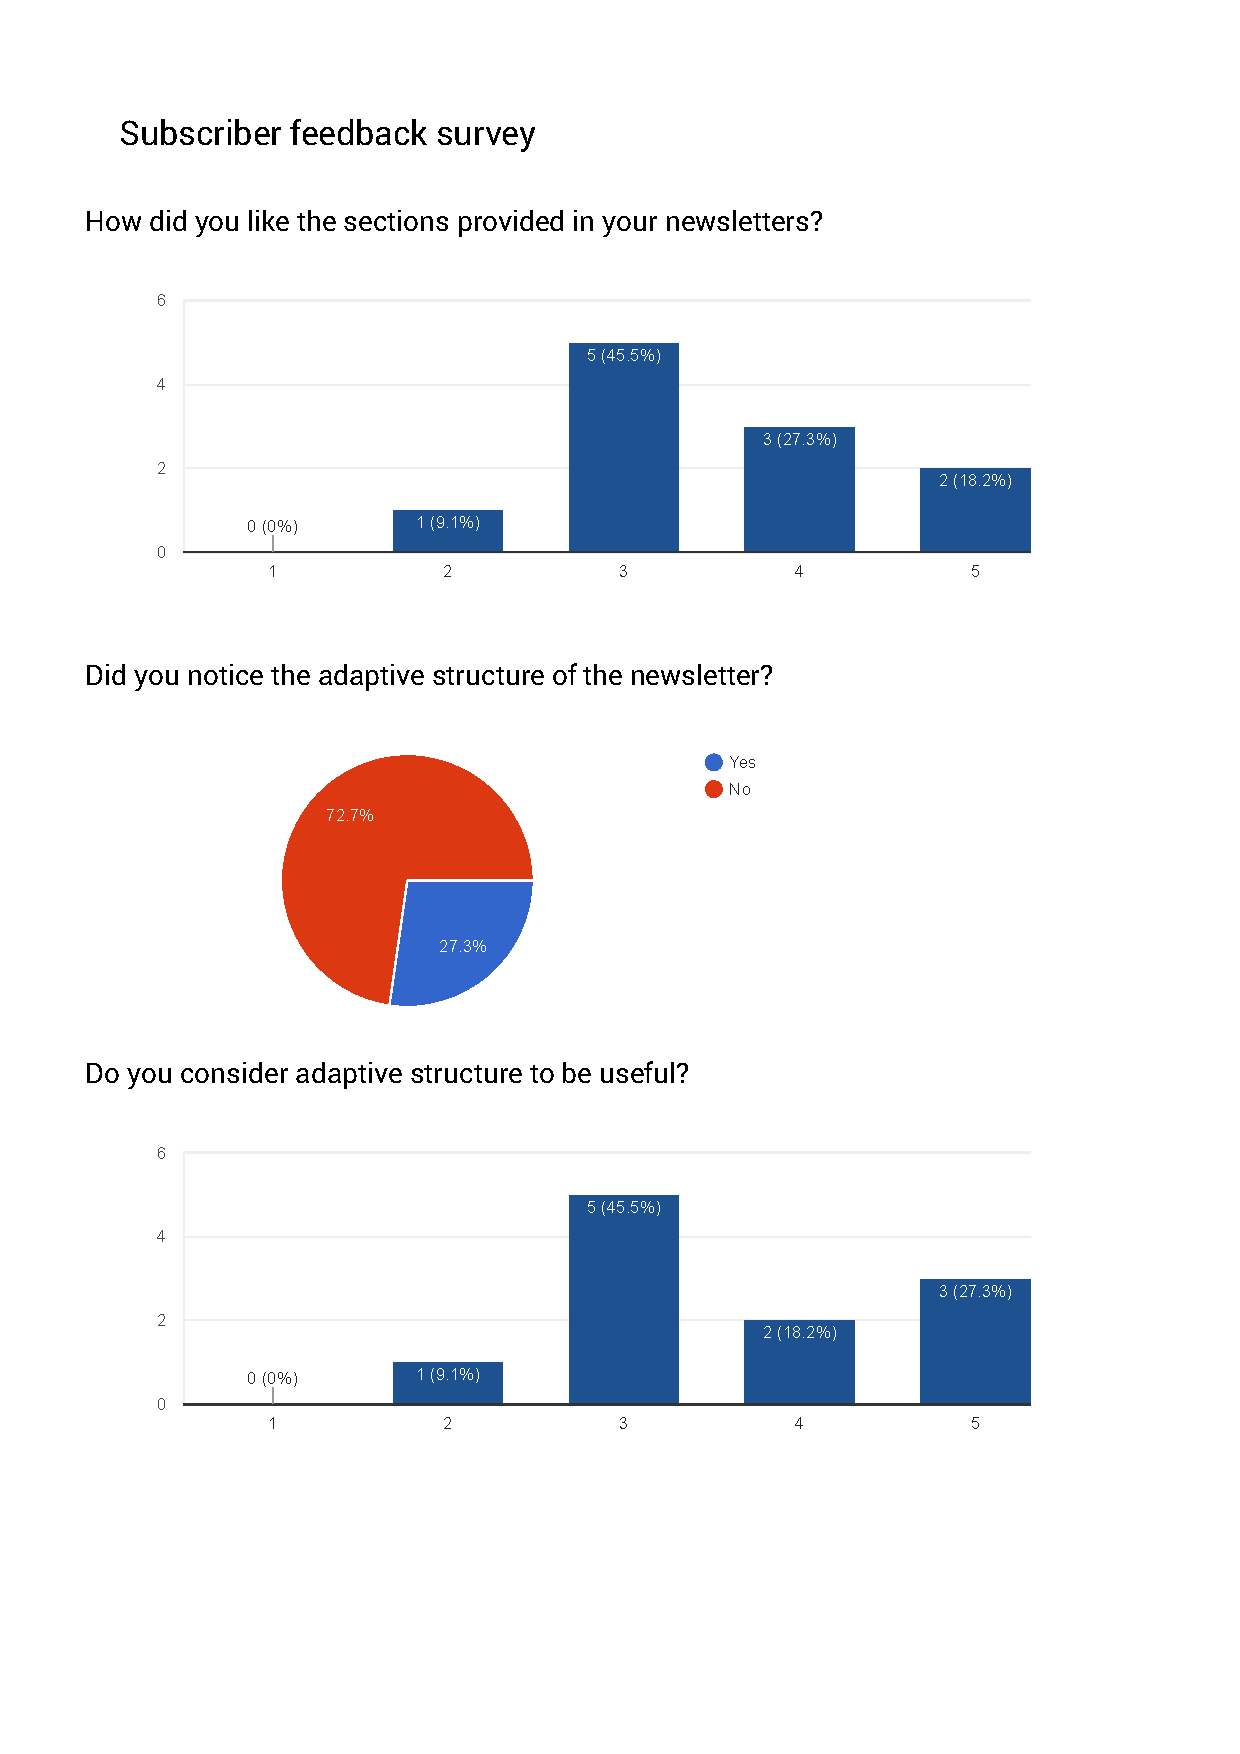
\includepdf[pages={1,2,3}, pagecommand={}, offset={0.45in -0.3in}]{figures/survey-results.pdf}


\chapter{Príspevok na konferencii IIT.SRC 2018}
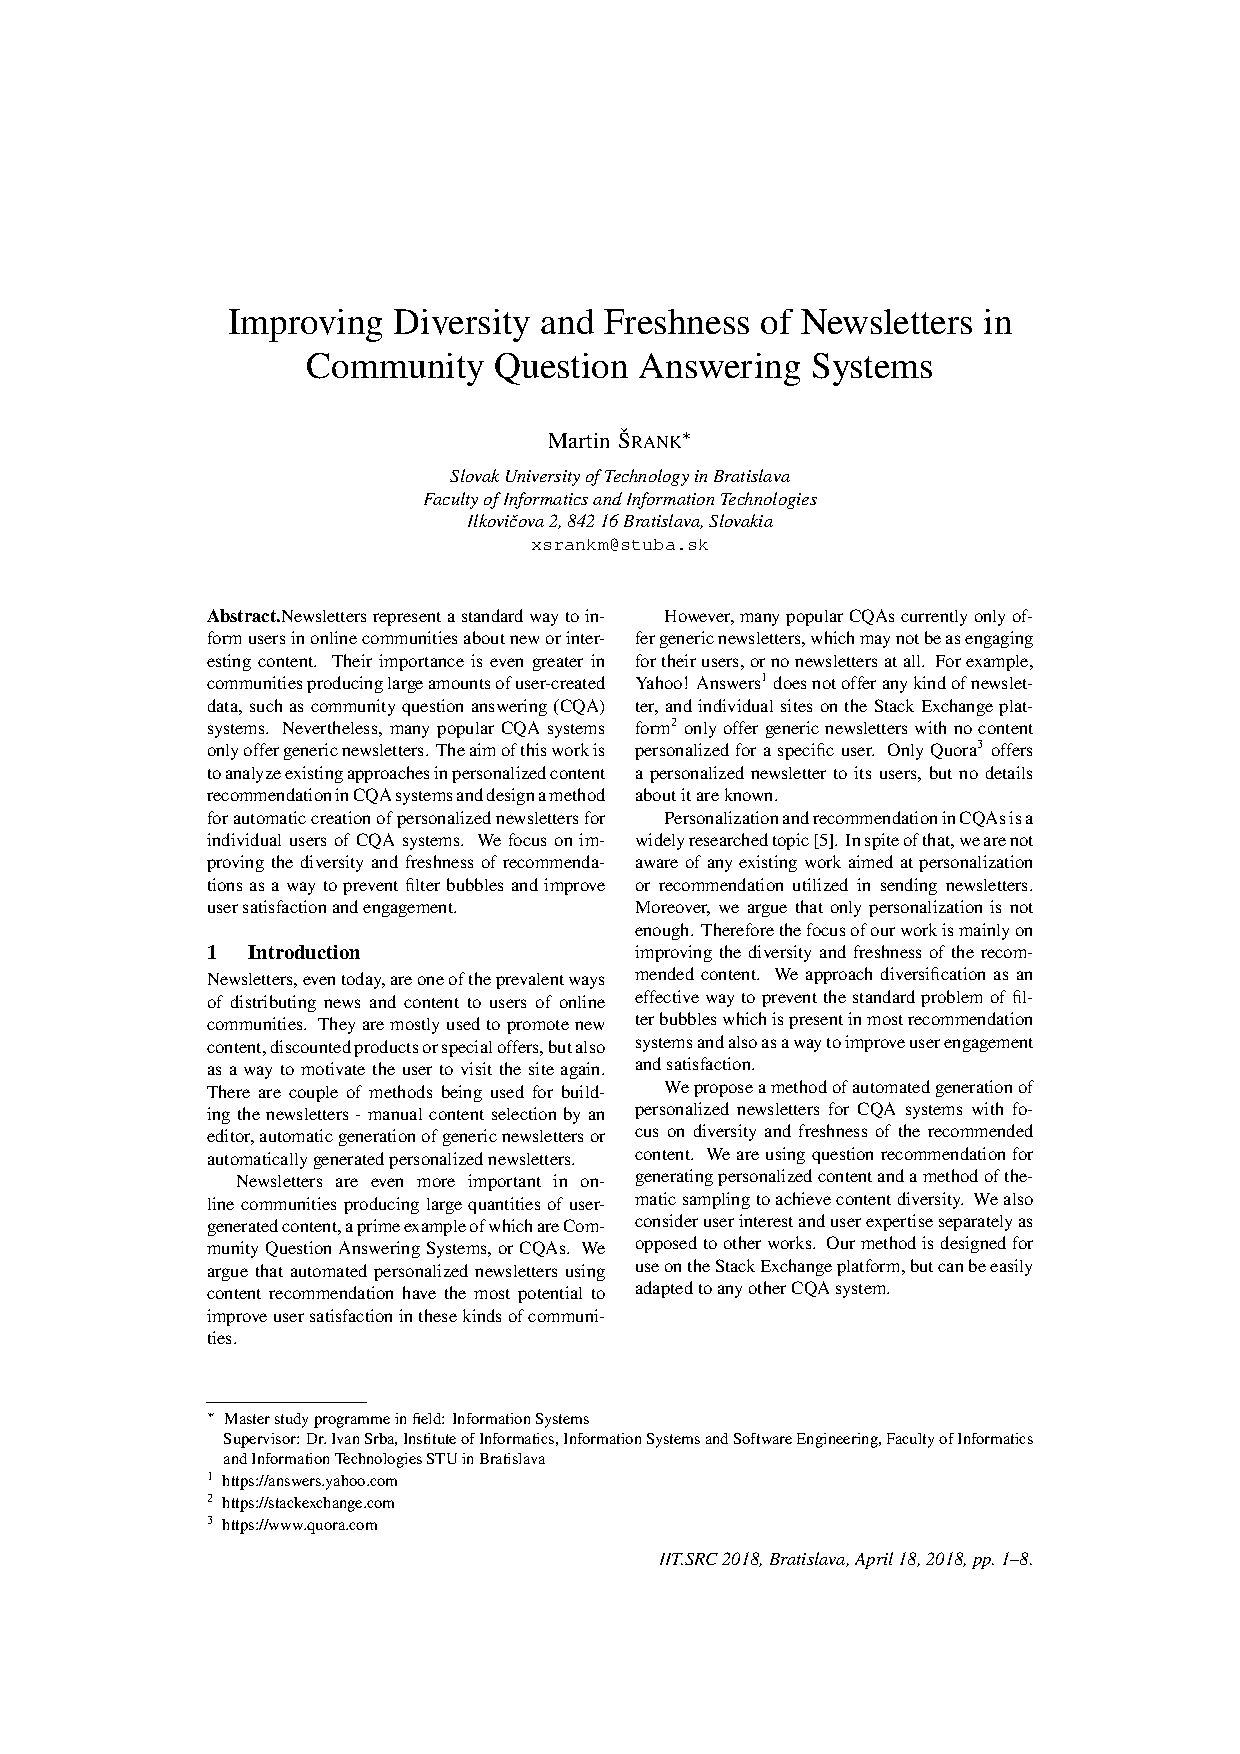
\includepdf[pages={1,2,3,4},pagecommand={}]{figures/iit-src.pdf}


\afterpage{\blankpage}
\newpage
\chapter{Elektronické médium}

Elektronické médium priložené k dokumentu má nasledovnú štruktúru:
\begin{my_itemize}
\emptyitem /code
	\begin{my_itemize}
	\myitem Zdrojové kódy samotných implementovaných modulov
	\end{my_itemize}
\emptyitem /doc
	\begin{my_itemize}
	\myitem Priebežná správa o riešení DP2 s~anotáciami v~slovenskom a~anglickom jazyku
	\end{my_itemize}
\emptyitem /doc/latex
	\begin{my_itemize}
	\myitem \LaTeX~zdrojové súbory dokumentácie
	\end{my_itemize}
\emptyitem /doc/bibtex
	\begin{my_itemize}
	\myitem BibTeX súbor s~použitými referenciami
	\end{my_itemize}
\emptyitem readme.txt
  \begin{my_itemize}
  \myitem opis obsahu elektronického média
  \end{my_itemize}
\end{my_itemize}
